\chapter{The problem}
\label{sec:problem}

\iffalse

Background definitions, notations, etc.
Problem definition
	- Relation to Helmholtz
Boundary condition
	- Sommerfeld
	- PML/ABC/DtN
Shifted Laplace operator


The Poisson problem:
	- Well behaved
	- Eigenvalues of the residual
	- Optimal method for finding solution

Helmholtz problem:
	- Misbehaved
	- Poor convergence
	- Indefinite discretisation matrix
\fi

The end goal is to solve the Helmholtz equation in cylindrical coordinates in an unbounded three-dimensional domain, with symmetry about the $z$-axis.
Simplifying slightly, we assume Dirichlet boundary conditions on all of the boundaries of the domain.
This removes the unboundedness of the domain for the purposes of testing the solver on the problem.
Exploiting the symmetry of the problem allows us to decompose the solution into its Fourier components and reduce the problem to two dimensions.

In this chapter, we will derive the formal statement of the problem starting from the wave equation.
Also included here is a discussion of the topics relevant to the practical solution of the problem.
The final outcome of this chapter should be the starting point for the finite element discretisation in chapter \ref{sec:fem}.




% ------------------------------

\section{Problem derivation}

Consider the three dimensional wave equation with wave speed $c$,
\begin{equation}
	\frac{1}{c^2} \frac{\partial^2 u(x,y,z,t)}{\partial t^2} = \nabla^2 u(x,y,z,t). \label{eqn:wave}
\end{equation}
As in \cite{oomph_hh}, we assume the existence of a separable solution where the time component of the solution is time-harmonic with frequency $\omega$,
we may write the real-valued solution as
\[
	u(x,y,z,t) = \Re \left( U(x,y,z)e^{-i\omega t} \right),
\]
where $U(x,y,z)$ is a complex-valued function.
Substituting this into \eqref{eqn:wave}, we obtain the Helmholtz equation
\begin{equation}
	\nabla^2 U(x,y,z) + k^2 U(x,y,z) = 0, \label{eqn:hh}
\end{equation}
where the wavenumber $k$ is defined as
\begin{align}
	k = \frac{\Omega}{c}.
\end{align}

The mapping between Cartesian coordinates $(x,y,z)$ and cylindrical polar coordinates $(r,\varphi,z)$ is given by
\begin{align}
	x &= r\cos(\varphi), \\
	y &= r\sin(\varphi), \\
	z &= z.
\end{align}
The Jacobian of this mapping is given by
\begin{align}
	J = \left\vert \frac{\partial(x,y,z)}{\partial(r,\varphi,z)} \right\vert = r. \label{eqn:cylindrical_mapping}
\end{align}
This mapping transforms our equation from $U(x,y,z)$ into $U(r,\varphi,z)$, 
which we may decompose into its Fourier components $u_N(r,z)$ around the $\varphi$ axis, so that
\begin{equation}
	U(r,\varphi,z) = \sum_{N=-\infty}^\infty u_N(r,z) e^{iN\varphi}. \label{eqn:full_eqn}
\end{equation}
By linearity of the Helmholtz equation, for each $N$, $u_N(r,z)$ must satisfy the Helmholtz equation.
This allows us to solve for each $N$ individually and then combine the solutions to form a full solution.

The Laplacian in cylindrical coordinates is given by
\begin{align}
	\nabla^2 = \frac{\partial^2 }{\partial r^2}
			 + \frac{1}{r} \frac{\partial }{\partial r}
			 + \frac{1}{r^2} \frac{\partial^2 }{\partial \varphi^2}
			 + \frac{\partial^2 }{\partial z^2}. \label{eqn:laplacian}
\end{align}
We also define the reduced Laplacian in cylindrical coordinates, consisting of only partial derivatives with respect to $r$ and $z$.
\begin{align}
	\nabla^2 = \frac{\partial^2 }{\partial r^2}
			 + \frac{1}{r} \frac{\partial }{\partial r}
			 + \frac{\partial^2 }{\partial z^2}. \label{eqn:laplacian_reduced}
\end{align}
It is not necessary to distinguish between the two operators \eqref{eqn:laplacian} and \eqref{eqn:laplacian_reduced}.
In the case of a function in $(r,\varphi,z)$, then the full cylindrical Laplacian is required.
Alternatively, for a function in $(r,z)$, the reduced cylindrical Laplacian is appropriate.
Therefore it should be implicit from the context of the equation.

Hence above, we wish to extract those terms consisting of $\varphi$ from \eqref{eqn:full_eqn}.
The partial derivatives with respect to $\varphi$ give
\begin{align}
	\frac{1}{r^2} \frac{\partial^2 }{\partial \varphi^2} \left( e^{i N \varphi}\right) = - \frac{N^2}{r^2} e^{i N \varphi}.
\end{align}
The full equation then becomes
\begin{align}
	\nabla^2 U(r,\varphi,z) 
		&= \nabla^2 \left[\sum_{N=-\infty}^\infty u_N(r,z) e^{i N \varphi}\right] \\
		&= \sum_{N=-\infty}^\infty \left[ 
										\nabla^2 u_N(r,z) - \frac{N^2}{r^2}u_N(r,z)
								   \right] e^{i N \varphi}.
\end{align}

Since we can solve each term in the series separately, we can extract a single equation for each $N$.
This gives us the Fourier decomposed Helmholtz equation,
\begin{equation}
	\nabla^2 u_N(r,z) + (k^2 - \frac{N^2}{r^2})u_N(r,z) = 0. \label{eqn:fhh}
\end{equation}

The standard Helmholtz equation is classified by a single parameter, the wavenumber $k$.
Decomposing the solution into Fourier components, we introduce the Fourier wavenumber $N$ as an additional parameter to the system.
These two parameters together determine the equation and thus the solutions for the problem.







% ----------------------------------------

\subsection{Multigrid for the Helmholtz equation}

There are difficulities in solving the Helmholtz equation using multigrid as the solver.
This is especially true for even moderate values of $k^2$.
Large values of $k^2$ cause the discretisation matrix to be indefinite, causing the solver to not converge.
Work has been done by several authors in order to overcome this shortcoming of multigrid \cite{cslp1, cslp2}.

Multigrid performs poorly for the Helmholtz equation due to the indefiniteness of the operator.
However, multigrid is a good solver for the nearby problem shifted into the complex plane.
This is not the problem we want to solve, but a good enough approximation to use as a preconditioner for another iterative method.

Introducing a shift to the complex plane, the Helmholtz operator in Cartesian coordinates becomes
\begin{align}
	\mathcal{L}_{CSLP} = \nabla^2 + (1 + i \alpha ) k^2,  \label{eqn:cslp}
\end{align}
where $\alpha$ is a positive real number controlling the offset from the real axis.

Since our equation is defined in Fourier decomposed cylindrical coordinates, we obtain 
\begin{align}
	\nabla^2 u_N(r,z) + \left[ \left( 1 + i \alpha \right) k^2 - \frac{N^2}{r^2} \right] u_N(r,z) = 0.
\end{align}
Here, the shift is still applied to the $k^2$ term, but we have the additional term from \eqref{eqn:fhh}.

The optimal value of $\alpha$ is determined in \cite{cslp2}.
Specifically, they state that taking $\alpha=0.5$ results in the best possible.
In all of our numerical experiments, we use this value for preconditioning FGMRES with multigrid.








% ----------------------------------------

\section{Related problems and other issues}

In the case where $k=0$, the problem reduces to the Poisson problem \eqref{eqn:poisson} with $f=0$, otherwise known as Laplace's equation.
Taking $k=0$ in equation \eqref{eqn:fhh}, we obtain
\begin{align}
	\nabla^2 U(r,\varphi,z) = \nabla^2 u_N(r,z) - \frac{N^2}{r^2} u_N(r,z) = 0. \label{eqn:fp}
\end{align}
This is Poisson's equation in Fourier decomposed cylindrical coordinates.

The Poisson equation is of interest because of the close relation between the Helmholtz and Poisson equations.
It is known that multigrid performs optimally for Poisson's equation.
Since we are interested in how multigrid performs when solving \eqref{eqn:fhh}, we will compare results with this equation.

Another related problem is the case when both $k=0$ and $N=0$.
This is the Poisson equation in reduced axisymmetric coordinates, where the solution depends only on $r$ and $z$.
To further aid in comparison between solutions, we will also consider how the equation behaves in this case.


% Variable coefficients --------------

A common issue arising when using a multigrid solver occurs with variable coefficient problems \cite{briggs}.
In Cartesian coordinates, the Helmholtz equation is a constant coefficient problem.
This is seen in the operator
\begin{align}
	\nabla^2 + k^2 = \frac{\partial^2}{\partial x^2} + \frac{\partial^2}{\partial t^2} + \frac{\partial^2}{\partial z^2} + k^2.
\end{align}

In cylindrical coordinates, however, we have a term that varies proportionally to the inverse of the radial distance squared.
For the Fourier decomposed Helmholtz equation, recall equation \eqref{eqn:fhh},
\begin{align}
	\frac{\partial^2 u_N}{\partial r^2}
			 + \frac{1}{r} \frac{\partial u_N}{\partial r}
			 + \frac{\partial^2 u_N}{\partial z^2}
			 + (k^2 - \frac{N^2}{r^2})u_N = 0. \label{eqn:full_fhh}
\end{align}
As suggested in \cite{briggs}, this may cause issues with multigrid.
A test of the method should be performed first to confirm before attempting to remedy potentially non-existent issues with variable coefficients.









% ----------------------------------------

\section{Domain and boundary conditions}

The full wave equation \eqref{eqn:wave} is defined in three spatial dimensions and one temporal dimension.
The full cylindrical Helmholtz equtation \eqref{eqn:full_eqn} is defined in a cylinder in three spatial dimensions.
If we let the cylindrical domain have a maximum radius of $R_{\mathrm{max}} > 0$, and let the domain contain a cylindrical cavity with some maximum radius $0<R_{\mathrm{min}}<R_\mathrm{max}$.
Then resulting domain is shown in figure \ref{fig:full_domain}.

In the reduced $(r,z)$ coordinates for the Fourier decomposed equation \eqref{eqn:fhh}, the domain becomes \ref{fig:reduced_domain}.
This simplification aids in the computational work by reducing the number of degrees of freedom of the problem.
It is only a matter of post-processing the solution to obtain the full 3D solution from the reduced computed solution, as nothing is lost due to symmetry.
To obtain the full domain from this, a rotation of $2\pi$ radians about the $z$-axis is performed.

To complete the problem formulation, boundary conditions must also be specified for the PDE.
The boundaries we need to specify on are the inner regions of the cylindrical walls.
This translates to the four boundaries in the reduced equation.
The Dirichlet boundary conditions on the entire boundary are then
\begin{align}
	u_N(r,z) = u_0 \quad \mathrm{on} \quad \partial \Omega,
\end{align}
for some given value of $u_0$.



\begin{figure}[ht!]
	% Need an example image of a 3d cylinder - the domain for the problem -- away from the 
	% Also the 2d section of the cylinder
	\centering
	\subfloat[][Full cylindrical domain. \label{fig:full_domain}]{
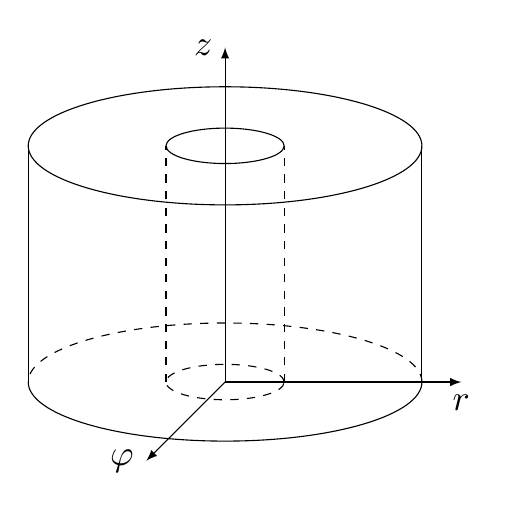
\begin{tikzpicture}[scale=2.5, >=latex]
  % AXES
  % z-axis
  \draw[->] (0.5,0) -- (0.5,1.7) node[left, scale=1.3] {$z$};
  % r-axis
  \draw[->] (0.5,0) -- (1.7,0) node[below, scale=1.3] {$r$};
  % phi-axis
  \draw[->] (0.5,0) -- (0.1,-0.4) node[left, scale=1.3] {$\varphi$};

  % INNER CYLINDER
  % top ellipse
  \draw[solid] (0.5,1.2) ellipse (0.3 and 0.09);
  % bottom ellipse
  \draw[dashed] (0.5,0) ellipse (0.3 and 0.09);
  
  % left line
  \draw[dashed] (0.2,0) -- ++(0,1.2);
  % right line
  \draw[dashed] (0.8,0) -- ++(0,1.2);


  % OUTER CYLINDER
  % top ellipse
  \draw[solid] (1.5,1.2) arc (0:180:1 and 0.3);
  \draw[solid] (-0.5,1.2) arc (180:360:1 and 0.3);
  % bottom ellipse
  \draw[dashed] (1.5,0) arc (0:180:1 and 0.3);
  \draw[solid] (-0.5,0) arc (180:360:1 and 0.3);
  
  % left line
  \draw (-0.5,0) -- ++(0,1.2);
  % right line
  \draw (1.5,0) -- ++(0,1.2);
\end{tikzpicture}	
	}\quad
	\subfloat[][Reduced dimensional domain. \label{fig:reduced_domain}]{
		\begin{tikzpicture}[scale=3, >=latex]
  % z-axis
  \draw[->] (0,0) -- ++(0,1.6) node[left, scale=1.3] {$z$};
  % r-axis
  \draw[->] (0,0) -- ++(1.7,0) node[below, scale=1.3] {$r$};

  \draw[solid] (0.3,0.15) -- ++(1,0) -- ++(0,1.2) -- ++(-1,0);
  \draw[dashed] (0.3,0.15) -- ++(0,1.2);

\end{tikzpicture}
	}
	\caption{Problem domain.\label{fig:problem_domain}}
\end{figure}









% --------------------------------------

\section{An analytical solution}

In order to show that the computed solution of a numerical method is producing accurate results, a known solution is required to validate results.
The 3D axisymmetric domain reduces to a 2D rectangle that sweeps around the $z$-axis.
Hence, we want to find an analytical solution on a rectangle in $r$ and $z$ coordinates.

Let us begin by assuming the existence of a separable solution,
\begin{align}
	u_N(r,z) = R(r)Z(z).
\end{align}
Substituting into \eqref{eqn:fhh}, we obtain
\begin{align}
	\left( \frac{\d^2 R(r)}{\d r^2} + \frac{1}{r} \frac{\d R(r)}{\d r} \right) Z(z) + \frac{\d^2 Z(z)}{\d z^2} R(r) + \left( k^2 - \frac{N^2}{r^2} \right) R(r) Z(z) = 0.
\end{align}
Dividing through by $R(r)Z(z)$, we can separate terms consisting of $r$ and $z$ on each side of the equation.
\begin{align}
	\left( \frac{\d^2 R(r)}{\d r^2} + \frac{1}{r} \frac{\d R(r)}{\d r} \right)\frac{1}{R(r)} + \left( k^2 - \frac{N^2}{r^2} \right) = - \frac{\d^2 Z(z)}{\d z^2} \frac{1}{Z(z)}.
\end{align}
Because both sides of this equation are equal expressions involving different variables, they must be equal to some constant, say $\lambda$, whose sign is yet to be determined.
Hence, we obtain two ordinary differential equations in $r$ and in $z$.
\begin{align}
	&\frac{\d^2 Z(z)}{\d z^2} + \lambda Z(z) = 0. \label{eqn:Z}\\
	&\frac{\d^2 R(r)}{\d r^2} + \frac{1}{r} \frac{\d R(r)}{\d r} + \left( k^2 + \lambda - \frac{N^2}{r^2} \right) R(r) = 0. \label{eqn:R}
\end{align}


First, we solve \eqref{eqn:R} for $R(r)$.
Consider the change of variables
\begin{align}
	\tilde{r} = r \sqrt{k^2 + \lambda}.
\end{align}
By the chain rule, derivatives in $\tilde{r}$ become
\begin{align}
	\frac{\d R}{\d r} &= \frac{\d \tilde{r}}{\d r} \frac{\d R}{\d \tilde{r}} = \sqrt{k^2 + \lambda} \frac{\d R}{\d \tilde{r}} \\
	\frac{\d^2 R}{\d r^2} &= \sqrt{k^2 + \lambda} \frac{\d}{\d \tilde{r}} \left[ \sqrt{k^2 + \lambda} \frac{\d R}{\d \tilde{r}} \right]
							= \left(k^2 + \lambda\right) \frac{\d^2 R}{\d \tilde{r}^2}
\end{align}
Substituting into \eqref{eqn:R}, 
\begin{align}
	\left(k^2 + \lambda\right) \frac{\d^2 R(\tilde{r})}{\d \tilde{r}^2} + 
	\frac{\left(k^2 + \lambda\right)}{\tilde{r}} \frac{\d R(\tilde{r})}{\d \tilde{r}} + 
	\left(k^2 + \lambda\right) \left( 1 - \frac{N^2}{\tilde{r}^2} \right) R(\tilde{r}) = 0.
\end{align}
Upon cancelling factors, we have the final equation, which may be recognised as Bessel's differential equation.
\begin{align}
	\frac{\d^2 R(\tilde{r})}{\d \tilde{r}^2} + 
	\frac{1}{\tilde{r}} \frac{\d R(\tilde{r})}{\d \tilde{r}} + 
	\left( 1 - \frac{N^2}{\tilde{r}^2} \right) R(\tilde{r}) = 0. \label{eqn:bessel_de}
\end{align}
The solution to \eqref{eqn:bessel_de} is a linear combination of Bessel functions of order $N$, and whose argument is $\tilde{r}=r \sqrt{k^2 + \lambda}$.
\begin{align}
	R(r) = c_1 J_N \left( r \sqrt{k^2 + \lambda} \right) + c_2 Y_N \left( r \sqrt{k^2 + \lambda} \right)
\end{align}


Now we turn to the solution of \eqref{eqn:Z}.
The form of the solution of $Z(z)$ is depending on the sign of $\lambda$.
Let $\mu$ be a positive real number.
If the sign is negative so that $\lambda=-\mu^2$, then $Z(z)$ is a linear combination of hyperbolic sine and cosine,
\begin{align}
	Z(z) = c_3 \sinh(\mu z) + c_4 \cosh(\mu z).
\end{align}
On the other hand, if the sign is positive, so that $\lambda=\mu^2$, then $Z(z)$ is a linear combination of sine and cosine,
\begin{align}
	Z(z) = c_3 \sin(\mu z) + c_4 \cos(\mu z).
\end{align}
Finally, if $\lambda=0$, then $Z(z)$ is the equation of a straight line,
\begin{align}
	Z(z) = c_3 z + c_4.
\end{align}

For the sake of simplicity, we can specify that $\lambda=0$.
We have then for the full general solution for a single Fourier mode,
\begin{align}
	u_N(r,z) = R(r)Z(z) = \left( c_1 J_N \left( k r \right) + c_2 Y_N \left( k r \right) \right) \left( c_3 z + c_4 \right),
\end{align}
for any given constants $c_1,c_2,c_4,c_4$.

Since the only purpose of this exact solution is for validation of a correct implementation, we may choose the constants above freely.
In doing so, we may then specify that the boundary conditions for the PDE must correspond with the exact solution.
That is, since we know a priori the solution of the equation, we let the boundary conditions be exactly the value of the solution on the boundary.
This has the benefit of finding the solution we have found above for us to check the method against.
Although this has the distinct disadvantage that we do not make use of any boundary conditions besides Dirichlet.
We will address this at a later with the introduction of Neumann and Sommerfeld boundary conditions.
